\chapter{Resultados}
El análisis de los resultados logrados es una de las partes finales obligatorias y conclusivas en la labor de investigación. En esta, procesamos la nueva información surgida como producto de la misma para presentarla de manera ordenada; tratando de conseguir la comprensión del lector y poder ligar los datos obtenidos a unas determinadas conclusiones.

En este capítulo de la memoria, realizaremos un pequeño análisis de las capacidades conseguidas en la implementación realizada para este estudio. Puesto que es complicada una interpretación objetiva de  una sensación tan subjetiva como lo es el tacto, trataremos en esta sección de poner de manifiesto el funcionamiento de la realimentación háptica lograda proporcionando información acerca de la misma. Para ello, realizaremos distintos test y pruebas comprobando así su eficacia y casos límite, exponiendo por medio de gráficas y el análisis de los valores que se toman en su funcionamiento. Así pues, en todo momento, trataremos de desarrollar una interpretación imparcial de los resultados obtenidos en base a los datos recogidos. 


\bigskip
\bigskip
\bigskip
\bigskip
\bigskip
\bigskip
\bigskip
\bigskip
\bigskip
\bigskip
\bigskip

\section{Benchmarks}
Se utiliza esta palabra, proveniente del inglés, para el designio de las comparativas de rendimiento cuyo objeto es el cotejo o testeo de los sistemas aludidos, de modo que nos permitan conocer en qué medida es bueno su funcionamiento o cuál es su grado de rendimiento respecto a unos valores fijados. 

De este modo, trataremos en esta sección de reflejar a través de distintos test el funcionamiento de las dos principales capacidades hápticas implementadas, como lo son la realimentación del momento de fuerza de los objetos prendidos por Baxter o la sensación de colisión con los mismos. 

\subsection{Gráficas de Evolución del Momento}
En primer lugar en este análisis, trataremos la implementación de la gravedad y el torque en el movimiento de un objeto simulado siendo agarrado por nuestro robot controlado. 

Así pues, como se explicó, un objeto posee un momento de fuerza o torque en el momento en que este se desplaza en relación a un punto de referencia con una cierta aceleración. Consecuentemente, extrapolándolo a nuestra propia experiencia, podemos sentir como al tomar un objeto y moverlo deliberadamente este ofrece una cierta resistencia a cambiar su estado de movimiento, sea para iniciarlo o para pararlo, teniendo que ejercer una fuerza en sentido contrario para ello.

Adicionalmente, la por todos conocida gravedad terrestre, impone a todos los cuerpos que caen bajo su acción un constante efecto de caída libre, empujando los mismos hacia su centro de gravedad con una de aceleración constante, mas no uniforme en todos sus puntos. Por ende, cada vez que sujetamos un objeto podemos sentir su peso, como consecuencia de la masa intrínseca en las entidades aludidas.

En el control de Baxter a través de Touch X, para esta sección de la investigación, hemos tratado de establecer un marco de pruebas controlado, en la medida de los posible, para que las mediciones realizadas sean claras y objetivas. Las gráficas que se muestran a continuación son el fruto de la toma de medidas en repetidas ocasiones para obtener valores promedios y representativos del conjunto total. En este caso, describimos la configuración para el testeo como una prueba de carácter real y que podría tener lugar en un escenario en el que nuestro robot realiza tareas de mantenimiento en el comentado ambiente de trabajo en IFMIF-DONES. Asimismo, Baxter tratará de desplazar en repetidas ocasiones un objeto real con 46.13 Kg de masa a través de los ejes X, Y, Z -figuras \ref{Fig:x_axis_baxter}, \ref{Fig:y_axis_baxter}, \ref{Fig:z_axis_baxter}- siendo controlado por un ser humano en todo el proceso. De este modo, aunque este no soporte dicha carga en un entorno real, queda patente la eficacia de la realimentación háptica que podría ser usada en cualquier otro dispositivo solamente modificando los mencionados parámetros de reescalado si fuese necesario.  


\begin{figure}[htb]
    \hfill
    \centering
   \begin{minipage}{0.33\textwidth}
    \centering
    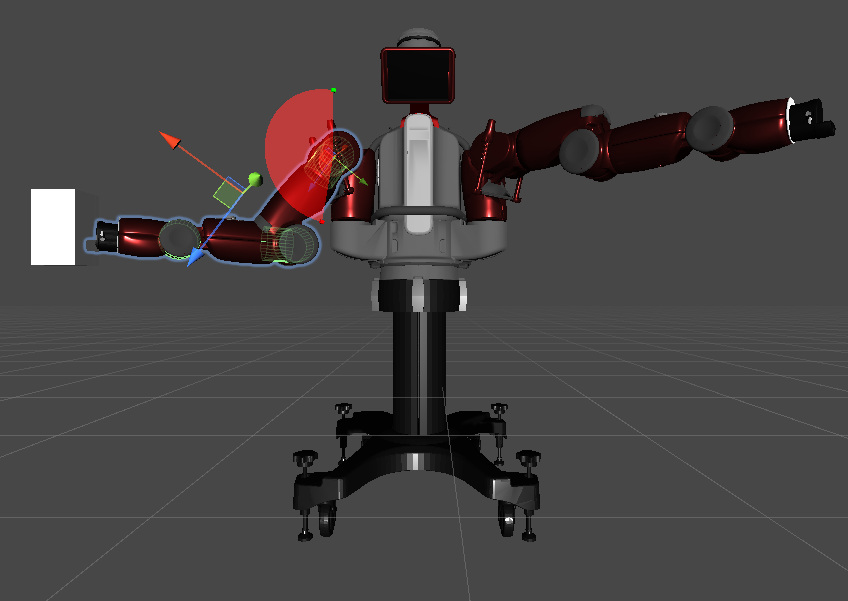
\includegraphics[width=0.9\textwidth]{imagenes/Baxter_Grabbing/FrontViewGrabbing.png}     
    \caption{}\label{Fig:x_axis_baxter}
   \end{minipage}\hfill
   \begin{minipage}{0.33\textwidth}
    \centering
    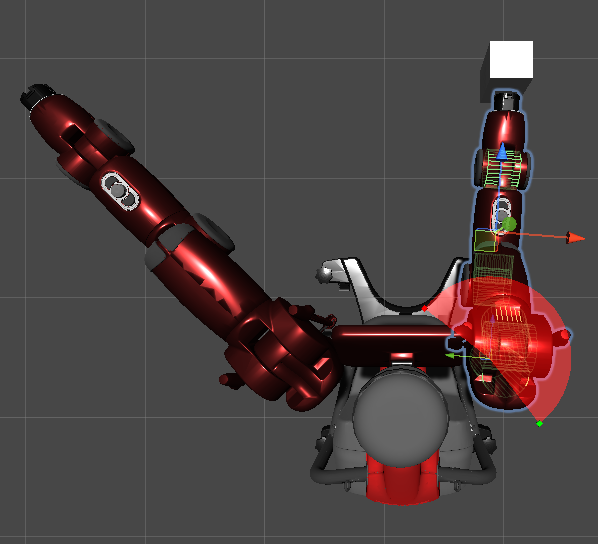
\includegraphics[width=0.8\textwidth]{imagenes/Baxter_Grabbing/TopViewGrabbing.png}     
    \caption{}\label{Fig:y_axis_baxter}
   \end{minipage}\hfill
   \begin{minipage}{0.34\textwidth}
    \centering
    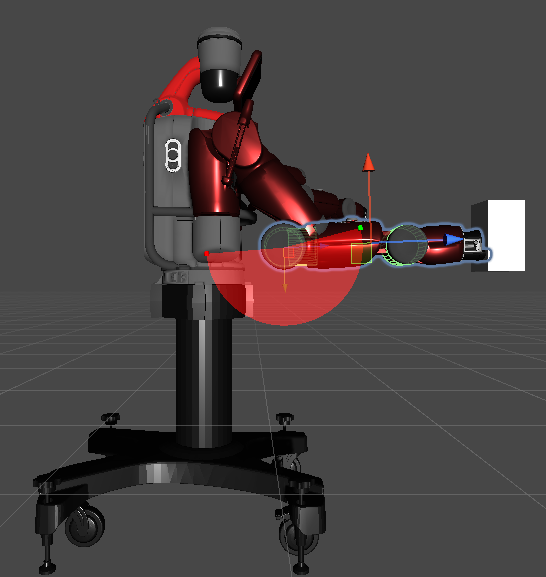
\includegraphics[width=0.7\textwidth]{imagenes/Baxter_Grabbing/LateralViewGrabbing.png}     
    \caption{}\label{Fig:z_axis_baxter}
   \end{minipage}
\end{figure}

Consecuentemente, monitorizaremos los valores establecidos para la simulación del comentado efecto y los representaremos de forma gráfica. En este caso, observaremos en ellas la evolución del torque frente al paso del tiempo en la simulación, medido en ms.

De igual manera, en el proceso de testeo, se lleva a cabo además el reajuste y refinamiento de algunos de los parámetros de reescalado que controlan algunos aspectos decisivos en la simulación de los citados efectos cinestésicos para que resulten lo más agradables al tacto, por lo que especificaremos en todo momento cuales son con exactitud.


\begin{figure}[htb]
   \begin{minipage}{0.33\textwidth}
     \centering
    \includesvg[width=1\textwidth]{imagenes/Mediciones_Torque/Sin_Filtro/Movimiento_en_X_frente_a_Tiempo.svg} 
    \caption{}\label{Fig:no_filter_pentration_test_x}
   \end{minipage}\hfill
   \begin{minipage}{0.33\textwidth}
     \centering
    \includesvg[width=1\textwidth]{imagenes/Mediciones_Torque/Sin_Filtro/Movimiento_en_Y_frente_a_Tiempo.svg} 
    \caption{}\label{Fig:no_filter_pentration_test_y}
   \end{minipage}
   \begin{minipage}{0.33\textwidth}
     \centering
    \includesvg[width=1\textwidth]{imagenes/Mediciones_Torque/Sin_Filtro/Movimiento_en_Z_frente_a_Tiempo.svg}     
    \caption{}\label{Fig:no_filter_pentration_test_z}
   \end{minipage}\hfill
\end{figure}

Los valores de escalado del momento y la gravedad son de 1.0, la ponderación de la misma en los ejes X, Y, Z resulta ser 1.0, 0.0, 0.0 respectivamente. Figuras \ref{Fig:no_filter_pentration_test_x},  \ref{Fig:no_filter_pentration_test_y},  \ref{Fig:no_filter_pentration_test_x}.

En esta primera serie de datos observamos los resultado en una ejecución en la que no establecemos ninguna compensación o comparativa con las fuerzas anteriormente calculadas. Como consecuencia, vemos como el rango en que se mueve la fuerza calculada es muy grande y algunos de los valores calculados muy pequeños, lo que resulta en una mala experiencia final por los golpes con un alto valor de fuerza repentinamente y los efectos de vibración. 

\bigskip
\bigskip
\bigskip
\bigskip
\bigskip


\begin{figure}[!hbt]
   \begin{minipage}{0.33\textwidth}
     \centering
    \includesvg[width=1\textwidth]{imagenes/Mediciones_Torque/Filtradas/Ponderacion_con_1/Movimiento_en_X_Media_ponderada_con_1.svg}     \caption{}\label{Fig:filtro_medias_1_x}
   \end{minipage}\hfill
   \begin{minipage}{0.33\textwidth}
     \centering
    \includesvg[width=1\textwidth]{imagenes/Mediciones_Torque/Filtradas/Ponderacion_con_1/Movimiento_en_Y_Media_ponderada_con_1.svg}     \caption{}\label{Fig:filtro_medias_1_y}
   \end{minipage}
   \begin{minipage}{0.33\textwidth}
     \centering
    \includesvg[width=1\textwidth]{imagenes/Mediciones_Torque/Filtradas/Ponderacion_con_1/Movimiento_en_Z_Media_ponderada_con_1.svg}     \caption{}\label{Fig:filtro_medias_1_z}
   \end{minipage}\hfill
\end{figure}

Los valores de escalado del momento y la gravedad son de 0.3, la ponderación de la misma en los ejes X, Y, Z resulta ser 1.0, 0.0, 0.0 respectivamente. Figuras \ref{Fig:filtro_medias_1_x},  \ref{Fig:filtro_medias_1_y},  \ref{Fig:filtro_medias_1_z}.

Con la sola comparación y promedio del torque actual y el anterior además del escalado en gravedad e inercia la mejora es palpable en la propia gráfica, ya que el rango de fuerzas en el que nos movemos resulta más comprensible por nuestro sentido del tacto. No obstante, aún fallan algunos aspectos como la gravedad, que resulta incómoda o poco precisa.

\begin{figure}[!htb]
   \begin{minipage}{0.33\textwidth}
     \centering
    \includesvg[width=1\textwidth]{imagenes/Mediciones_Torque/Filtradas/Ponderacion_con_2/Movimiento_en_X_Media_ponderada_con_2.svg}     \caption{ }\label{Fig:filtro_medias_2_x}
   \end{minipage}\hfill
   \begin{minipage}{0.33\textwidth}
     \centering
    \includesvg[width=1\textwidth]{imagenes/Mediciones_Torque/Filtradas/Ponderacion_con_2/Movimiento_en_Y_Media_ponderada_con_2.svg}     \caption{ }\label{Fig:filtro_medias_2_y}
   \end{minipage}
   \begin{minipage}{0.33\textwidth}
     \centering
    \includesvg[width=1\textwidth]{imagenes/Mediciones_Torque/Filtradas/Ponderacion_con_2/Movimiento_en_Z_Media_ponderada_con_2.svg}     \caption{ }\label{Fig:filtro_medias_2_z}
   \end{minipage}\hfill
\end{figure}

Los valores de escalado del momento y la gravedad son de 0.2, la ponderación de la misma en los ejes X, Y, Z resulta ser 0.7, 0.0, 0.1 respectivamente. Figuras \ref{Fig:filtro_medias_2_x},  \ref{Fig:filtro_medias_2_y},  \ref{Fig:filtro_medias_2_z}.

En este punto observamos que la gravedad resulta más agradable al tacto, aunque los cambios en el momento de fuerza aún son imprecisos y la ponderación de la gravedad inadecuada. Sin embargo, podemos observar como en cada oscliación en el control a través de Touch X se producen crestas de fuerza, que es el comportamiento esperado. 

\begin{figure}[!htb]
   \begin{minipage}{0.33\textwidth}
     \centering
    \includesvg[width=1\textwidth]{imagenes/Mediciones_Torque/Filtradas/Ponderacion_con_4/Movimiento_en_X_Media_ponderada_con_4.svg}     \caption{ }\label{Fig:filtro_medias_4_x}
   \end{minipage}\hfill
   \begin{minipage}{0.33\textwidth}
     \centering
    \includesvg[width=1\textwidth]{imagenes/Mediciones_Torque/Filtradas/Ponderacion_con_4/Movimiento_en_Y_Media_ponderada_con_4.svg}     \caption{ }\label{Fig:filtro_medias_4_y}
   \end{minipage}
   \begin{minipage}{0.33\textwidth}
     \centering
    \includesvg[width=1\textwidth]{imagenes/Mediciones_Torque/Filtradas/Ponderacion_con_4/Movimiento_en_Z_Media_ponderada_con_4.svg}     \caption{ }\label{Fig:filtro_medias_4_z}
   \end{minipage}\hfill
\end{figure}


\begin{figure}[!htb]
   \begin{minipage}{0.33\textwidth}
     \centering
    \includesvg[width=1\textwidth]{imagenes/Mediciones_Torque/Filtradas/Ponderacion_con_8/Movimiento_en_X_Media_ponderada_con_8.svg}     \caption{ }\label{Fig:filtro_medias_8_x}
   \end{minipage}\hfill
   \begin{minipage}{0.33\textwidth}
     \centering
    \includesvg[width=1\textwidth]{imagenes/Mediciones_Torque/Filtradas/Ponderacion_con_8/Movimiento_en_Y_Media_ponderada_con_8.svg}     \caption{ }\label{Fig:filtro_medias_8_y}
   \end{minipage}
   \begin{minipage}{0.33\textwidth}
     \centering
    \includesvg[width=1\textwidth]{imagenes/Mediciones_Torque/Filtradas/Ponderacion_con_8/Movimiento_en_Z_Media_ponderada_con_8.svg}     \caption{ }\label{Fig:filtro_medias_8_z}
   \end{minipage}\hfill
\end{figure}

Los valores de escalado del momento y la gravedad son de 0.2, la ponderación de la misma en los ejes X, Y, Z resulta ser 0.9, 0.0, 0.1 respectivamente. Figuras \ref{Fig:filtro_medias_4_z},  \ref{Fig:filtro_medias_4_y},  \ref{Fig:filtro_medias_4_z}, \ref{Fig:filtro_medias_8_x},  \ref{Fig:filtro_medias_8_y},  \ref{Fig:filtro_medias_8_z}.

Advertimos que el filtro de medias de orden x respecto al torque escala correctamente, percibiendo mejoras tanto en los gráficos como en la realimentación háptica proporcionada . De este modo, notamos que los resultados obtenidos comienzan a asemejarse a funciones matemáticas concocidas. Además podemos ver como la gravedad se representa el eje X, apreciándose un torque constante y negativo en el mismo.

\begin{figure}[!htb]
   \begin{minipage}{0.33\textwidth}
     \centering
    \includesvg[width=1\textwidth]{imagenes/Mediciones_Torque/Filtradas/Ponderacion_con_10/Movimiento_en_X_Media_ponderada_con_10.svg}     \caption{ }\label{Fig:filtro_medias_10_x}
   \end{minipage}\hfill
   \begin{minipage}{0.33\textwidth}
     \centering
    \includesvg[width=1\textwidth]{imagenes/Mediciones_Torque/Filtradas/Ponderacion_con_10/Movimiento_en_Y_Media_ponderada_con_10.svg}     \caption{ }\label{Fig:filtro_medias_10_y}
   \end{minipage}
   \begin{minipage}{0.33\textwidth}
     \centering
    \includesvg[width=1\textwidth]{imagenes/Mediciones_Torque/Filtradas/Ponderacion_con_10/Movimiento_en_Z_Media_ponderada_con_10.svg}     \caption{ }\label{Fig:filtro_medias_10_z}
   \end{minipage}\hfill
\end{figure}

Los valores de escalado del momento y la gravedad son de 0.2, la ponderación de la misma en los ejes X, Y, Z resulta ser 0.9, 0.0, 0.1 respectivamente. Figuras \ref{Fig:filtro_medias_10_x},  \ref{Fig:filtro_medias_10_y},  \ref{Fig:filtro_medias_10_z}.

Tras la realización de esta ingente cantidad de pruebas notamos que el feedback cinestésico es bastante bueno y se asemeja a la implementación de los complementos desarrollados por parte de 3DSystems, compañía creadora del dispositivo. En este caso podemos ver como la función obtenida toma una forma sinusoidal, debida en cierto modo al balanceo en el testeo.

\bigskip
\bigskip
\bigskip
\bigskip
\bigskip
\bigskip
\bigskip
\bigskip
\bigskip
\bigskip

\begin{figure}[!htb]
   \begin{minipage}{0.33\textwidth}
     \centering
    \includesvg[width=1\textwidth]{imagenes/Mediciones_Torque/Filtradas/Ponderacion_con_12/Movimiento_en_X_Media_ponderada_con_12.svg}     \caption{ }\label{Fig:filtro_medias_12_x}
   \end{minipage}\hfill
   \begin{minipage}{0.33\textwidth}
     \centering
    \includesvg[width=1\textwidth]{imagenes/Mediciones_Torque/Filtradas/Ponderacion_con_12/Movimiento_en_Y_Media_ponderada_con_12.svg}     \caption{ }\label{Fig:filtro_medias_12_y}
   \end{minipage}
   \begin{minipage}{0.33\textwidth}
     \centering
    \includesvg[width=1\textwidth]{imagenes/Mediciones_Torque/Filtradas/Ponderacion_con_12/Movimiento_en_Z_Media_ponderada_con_12.svg}     \caption{ }\label{Fig:filtro_medias_12_z}
   \end{minipage}\hfill
\end{figure}
Los valores de escalado del momento y la gravedad son de 0.2, la ponderación de la misma en los ejes X, Y, Z resulta ser 0.9, 0.0, 0.1 respectivamente. Figuras \ref{Fig:filtro_medias_12_x},  \ref{Fig:filtro_medias_12_y},  \ref{Fig:filtro_medias_12_z}.

Finalmente intuimos que llegamos a un máximo en el escalado de esta técnica. En este caso, la realimentación proporcionada ya no es tan agradable al tacto y resulta confusa en algunos casos. Además de ello los cambios en el sentido de la fuerza resultan excéntricos resultando en pérdidas en los extremos.

Tras las distintas pruebas realizadas decidimos hacer uso de media móvil de orden 10 \cite{80}, lo que favorecerá la estabilidad en el desarrollo de actividades que impliquen su uso y dificultará los cambios bruscos en las mismas. Este valor es elegido tras la valoración de los gráficos expuestos y la sensación en la propia mano en el testeo. En perspectiva este no es un valor muy alto, ya que la función encargada de actualizar los valores del momento o de la gravedad se ejecuta en cada frame, y los frames tienen lugar entre 60 y 80 veces por segundo en nuestro equipo. A ese respecto, una nota importante a considerar es que la potencia del equipo puede afectar en gran medida al renderizado de la retroalimentación háptica, ya que en los casos en que se utilizaba una alta resolución para la visualización de las cámaras en el desarrollo de la prueba podíamos notar cierta cadencia en la misma.

En conclusión, cabe destacar que las pruebas han sido llevado a cabo por un ser humano, lo que hace que tengan un carácter más real. No obstante, al no hacer un manejo totalmente exacto del dispositivo podemos haber introducido, una pequeña cantidad de ruido.

\subsection{Gráficas de Evolución de Torque en Colisión}
Continuando pues con el testeo de las funcionalidades desarrolladas, trataremos en este apartado la evolución del torque que sentiremos en la colisión con los distintos objetos con los que el robot controlado puede interactuar en la simulación o, en una fase más avanzada, en el mundo real.

De este modo, como reseñamos anteriormente, en el momento en que tratamos de realizar una fuerza para tratar de cambiar el estado de reposo de un cuerpo, hace acto de presencia una fuerza normal que interpretamos como una aparente resistencia por parte del mismo en sentido contrario, que en consecuencia a la extensión del brazo de Baxter se manifestará como un torque que deberemos reflejar. 

Consecuentemente, podemos ejemplificar este hecho con un caso cotidiano de uso como es el apretar una simple tuerca haciendo uso de una llave inglesa. En este caso aplicamos una fuerza en su extremo que, a causa de la distancia al punto de referencia -el propio perno-, resultará en un torque aplicado. 

Al igual que en la experimentación y testeo en el apartado anterior, en este caso se trata de establecer un ambiente de pruebas realista a la par que lo más pulcro posible. De este modo, los resultados que presentamos dimanan de los ensayos iterativos y la toma de medidas en promedio de las susodichas pruebas realizadas. Así pues, tomaremos nota de la evolución de la fuerza al tratar de atravesar un objeto simulado como inamovible en los ejes X, Y, Z de la forma que ejemplifican las figuras \ref{Fig:FrontViewCollidingX},  \ref{Fig:FrontViewCollidingY},  \ref{Fig:LateralViewCollidingZ} respectivamente.

\begin{figure}[htb]
	\hfill
	\centering
	\begin{minipage}{0.33\textwidth}
		\centering
		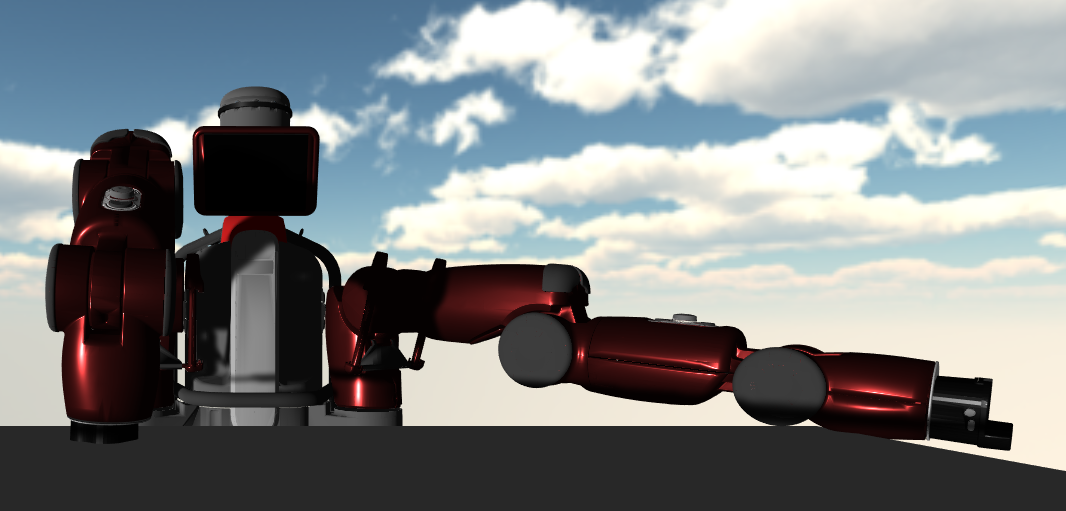
\includegraphics[width=0.8\textwidth]{imagenes/Baxter_Colliding/FrontViewCollidingX.png}     
		\caption{}\label{Fig:FrontViewCollidingX}
	\end{minipage}\hfill
	\begin{minipage}{0.33\textwidth}
		\centering
		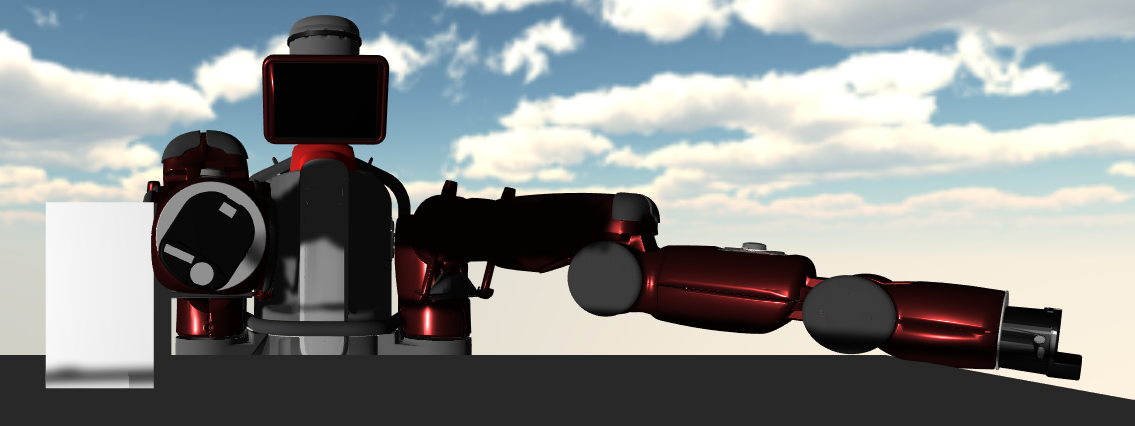
\includegraphics[width=1\textwidth]{imagenes/Baxter_Colliding/FrontViewCollidingY.png}     
		\caption{}\label{Fig:FrontViewCollidingY}
	\end{minipage}\hfill
	\begin{minipage}{0.34\textwidth}
		\centering
		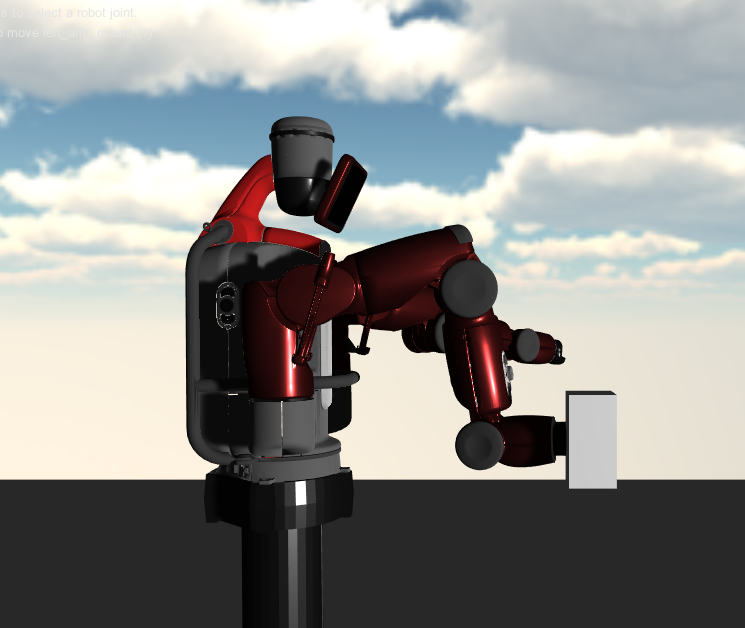
\includegraphics[width=0.6\textwidth]{imagenes/Baxter_Colliding/LateralViewCollidingZ.png}     
		\caption{}\label{Fig:LateralViewCollidingZ}
	\end{minipage}
\end{figure}

La  función que seguirán las intensidades de la realimentación háptica es la ya comentada exponencial, definida en el epígrafe dedicado a la implementación. Asimismo, la función teórica diseñada posee la característica de poder especificar, dependiendo del parámetro divisor del logaritmo, el valor en el que se alcanzará el valor máximo de torque especificado en metros. Por ende, haremos pruebas de ejecución variando este factor representando en este caso los valores de torque -en mNm- que se asocian a distintas intensidades de penetración, que mediremos en cm. 

\begin{figure}[!htb]
	\begin{minipage}{0.33\textwidth}
		\centering
		\includesvg[width=1\textwidth]{imagenes/Medidas_Colision/10/Torque_frente_a_ Penetracion_en_X_Maximo_10.svg}     \caption{ }\label{Fig:penetracion_x_maximo_10}
	\end{minipage}\hfill
	\begin{minipage}{0.33\textwidth}
		\centering
		\includesvg[width=1\textwidth]{imagenes/Medidas_Colision/10/Torque_frente_a_ Penetracion_en_Y_Maximo_10.svg}     \caption{ }\label{Fig:penetracion_y_maximo_10}
	\end{minipage}
	\begin{minipage}{0.33\textwidth}
		\centering
		\includesvg[width=1\textwidth]{imagenes/Medidas_Colision/10/Torque_frente_a_ Penetracion_en_Z_Maximo_10.svg}     \caption{ }\label{Fig:penetracion_z_maximo_10}
	\end{minipage}\hfill
\end{figure}

\begin{figure}[!htb]
	\begin{minipage}{0.33\textwidth}
		\centering
		\includesvg[width=1\textwidth]{imagenes/Medidas_Colision/20/Torque_frente_a_ Penetracion_en_X_Maximo_20.svg}     \caption{ }\label{Fig:penetracion_x_maximo_20}
	\end{minipage}\hfill
	\begin{minipage}{0.33\textwidth}
		\centering
		\includesvg[width=1\textwidth]{imagenes/Medidas_Colision/20/Torque_frente_a_ Penetracion_en_Y_Maximo_20.svg}     \caption{ }\label{Fig:penetracion_y_maximo_20}
	\end{minipage}
	\begin{minipage}{0.33\textwidth}
		\centering
		\includesvg[width=1\textwidth]{imagenes/Medidas_Colision/20/Torque_frente_a_ Penetracion_en_Z_Maximo_20.svg}     \caption{ }\label{Fig:penetracion_z_maximo_20}
	\end{minipage}\hfill
\end{figure}

Observamos resultados similares a la curva teórica de evolución prevista en los valores obtenidos. En este caso mostramos la evolución del torque para una penetración máxima establecida de 10 cm en, \ref{Fig:penetracion_x_maximo_10},  \ref{Fig:penetracion_y_maximo_10},  \ref{Fig:penetracion_z_maximo_10}, y de 20 cm para \ref{Fig:penetracion_x_maximo_20},  \ref{Fig:penetracion_y_maximo_20},  \ref{Fig:penetracion_z_maximo_20}. De igual manera, podemos ver como las gráficas difieren en su colocación pero se conserva la forma, denotando que se respeta la función implementada. Este efecto se debe a que el torque en el dispositivo háptico, y la penetración trazada de las articulaciones, se representan con valores positivos o negativos en cada caso, permitiendo inferir a través del signo asociado el sentido del desplazamiento que se realiza. Adicionalmente, es visible en los gráficos el valor máximo fijado para el torque que sentimos en el límite dispuesto, ya que valores más altos pueden desestabilizar el dispositivo y hacer que el operario, por error, lo haga caer.

Finalmente, atisbamos en la ejecución de las pruebas que una evolución más paulatina gracias al factor corrector en 20 cm hace que el efecto sea más agradable al tacto, postulándose este valor como el más idóneo entre ambos. Así mismo, como en apartados anteriores, para la corrección de ruido hacemos uso de la media móvil, que suavizará los efectos transmitidos pese a cobrar una menor importancia en esta actividad. Adicionalmente, cabe destacar que la penetración medida no resultará en ningún momento en una incursión por parte del robot real en ninguno de los objetos manipulados, ya que esta es meramente una medida virtual utilizada para el cálculo de la resistencia que ofrecemos. A tal efecto, gracias a esta implementación asistiremos al manipulador remoto para no dañar a Baxter o su entorno de trabajo, ya que tendrá consciencia en todo momento de si está o no colisionando.

